The shadow suppression is performed in a fashion similar to what is mentioned in the paper by Woods \cite{Wood}. The suppression if performed using the Hue- Saturation- Value- (HSV) mapping, The HSV mapping was chosen since it gives very small amounts of false positives (non shadow pixels labeled as shadow pixels) and a manageable number of false negatives, while at the same time being fairly simple. We make the assumption that a if a pixel is shadowed the hue remains constant, while there is a decrease in both the value and saturation channels compared to the most likely background at the time. To test the performance of the shadow suppression, the Renova footage produced in the IVSS project at CVL Linköping University was used. 


\subsubsection{Implementation}
The Shadow Suppression function is called with a reference to \emph{frame} object containing both a processed version of the probability map, the current frame image as well as the most likely background. The first step is to remap the current frame image and the background model to the HSV-space. The suppression is performed by comparing all H- S- and V-values in the remapped images. If a pixel marked as foreground by the background model has a the same hue but lower saturation and value in the image than in the background model, it is assumed to be caused by a shadow, (eq. 3.19 in \cite{Wood}). All probability map pixels assumed to be shadows are set to zero, and the shadow suppression is thereby finished.

\subsubsection{Parameters}
The parameters that need to be specified in the shadow suppression are the threshold values for the different channels, $\tau_H$, $\tau_S$, $\alpha$ and $\beta$. Let i denote the current image and m the currently most probable background. In order for a pixel to be classified as shadow, all of the following three constraints have to be fulfilled:

\begin{equation}
	|H_i - H_m| < \tau_H
	\label{eq:H}
\end{equation}
\begin{equation}
	S_i - S_m < \tau_S
	\label{eq:S}
\end{equation}
\begin{equation}
	\alpha < \frac{V_i}{V_m} < \beta
	\label{eq:V}
\end{equation}

The parameter setting depend on the scene that is being observed. For example in figure \ref{fig:shadow_suppression_R0002_fig} where most of the shadows are cast on a gray road (hue $\approx 0$), a rather large $\tau_H$ is required. Also, since the shadows are not so profound, alpha can be raised, causing lower false positives for dark objects. There are big problems with false positives from the shadow suppression on dark objects, for example the car windows in the Renova 0000 sequence (figure \ref{fig:shadow_suppression_R0000_fig}). This can also be seen to some extent in figure \ref{fig:shadow_suppression_R0002_fig}, from the Renova 0002 sequence. These two figures illustrate how the parameters have to be changed, especially $\alpha$, when the lighting conditions vary over time. Even though $\alpha$ is significantly lower in figure \ref{fig:shadow_suppression_R0000_fig}, we still get shadow pixel labeled as foreground near the car in the middle of the image.

\newpage
\begin{figure}[h]
	\centering
	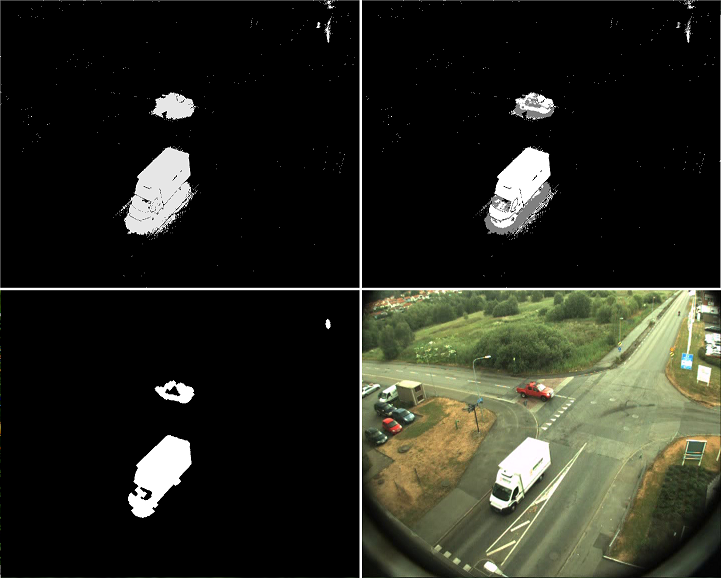
\includegraphics[width=\linewidth]{images/ShadowRenova0002.png}
	\caption{\textit{Renova image sequence 0002, frame 217. 
	\newline
	Top row: Background model output, model output with marked shadow pixels (gray) 
	\newline
	Bottom row: final foreground image, actual video frame.}}
	\label{fig:shadow_suppression_R0002_fig}  %Skapar referens till figuren
\end{figure}
Note that the moped is classified as shadow (false positive) and that the white dot in the upper right corner is created by the flag moving in the wind.\\

The parameters used to create the images in figure \ref{fig:shadow_suppression_R0002_fig} above were:

\begin{table}[h]
\centering
\begin{tabular}{|c|c|}
	\hline
	Parameter & Value  \\
	\hline
	$\tau_H$ &  0.2 \\
	\hline
	$\tau_S$ & 0.5 \\
	\hline
	$\alpha$ &  0.5 \\
	\hline
	$\beta$ &  0.95 \\
	\hline
\end{tabular}
\caption{\textit{Parameters used to create figure \ref{fig:shadow_suppression_R0002_fig}.}}
\label{tab:shadow_parameters_R0002_fig}
\end{table}

\newpage
\begin{figure}[htb]
	\centering
	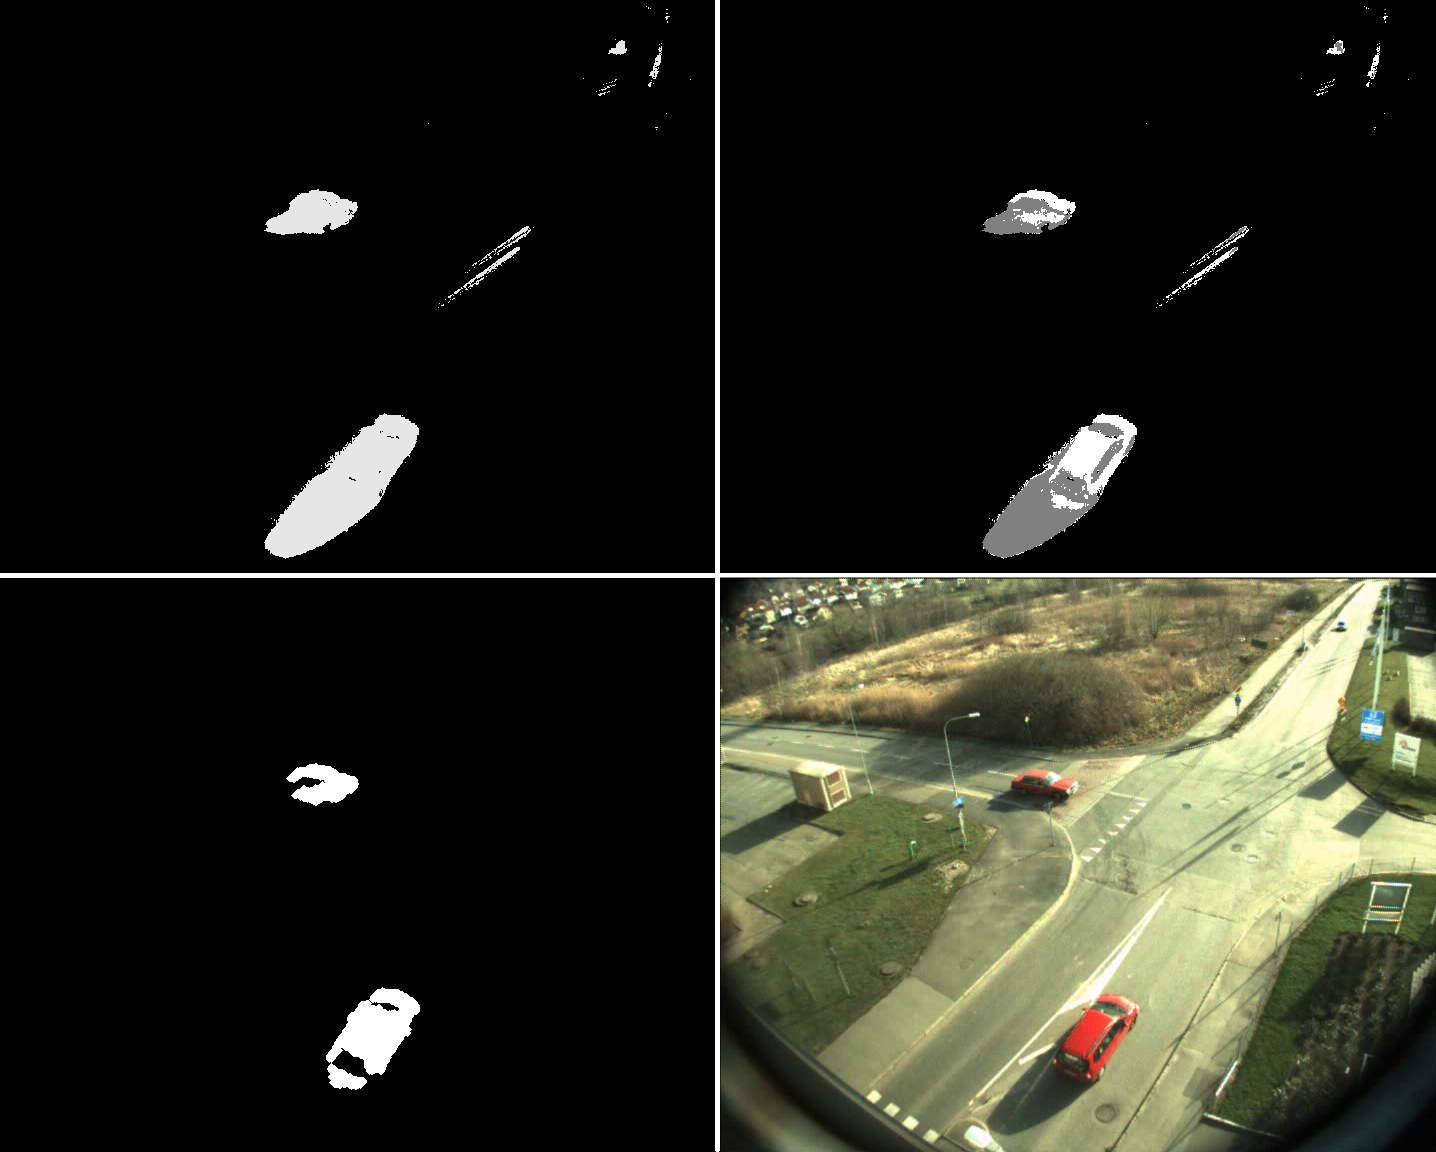
\includegraphics[width=\linewidth]{images/ShadowRenova0000.png}
	\caption{\textit{Renova image sequence 0000, frame 209. 
	\newline
	Top row: Background model output, model output with marked shadow pixels (gray)
	\newline
	Bottom row: final foreground image, actual video frame.}}
	\label{fig:shadow_suppression_R0000_fig}  %Skapar referens till figuren
\end{figure}
Note the false positives on the car windows and the dark regions on the approaching vehicle.

The parameters used to create the images in figure \ref{fig:shadow_suppression_R0000_fig} above were:

\begin{table}[htb]
\centering
\begin{tabular}{|c|c|}
	\hline
	Parameter & Value  \\
	\hline
	$\tau_H$ &  0.5 \\
	\hline
	$\tau_S$ & 0.5 \\
	\hline
	$\alpha$ &  0.3 \\
	\hline
	$\beta$ &  0.95 \\
	\hline
\end{tabular}

\caption{\textit{Parameters used to create figure \ref{fig:shadow_suppression_R0000_fig}.}}
\label{tab:shadow_parameters_R0000}
\end{table}
